\documentclass[compress,red]{beamer}
\mode<presentation>

\usetheme{Warsaw}

% other themes: AnnArbor, Antibes, Bergen, Berkeley, Berlin, Boadilla, boxes, CambridgeUS, Copenhagen, Darmstadt, default, Dresden, Frankfurt, Goettingen,
% Hannover, Ilmenau, JuanLesPins, Luebeck, Madrid, Maloe, Marburg, Montpellier, PaloAlto, Pittsburg, Rochester, Singapore, Szeged, classic

%\usecolortheme{lily}
% color themes: albatross, beaver, beetle, crane, default, dolphin, dov, fly, lily, orchid, rose, seagull, seahorse, sidebartab, structure, whale, wolverine

%\usefonttheme{serif}
% font themes: default, professionalfonts, serif, structurebold, structureitalicserif, structuresmallcapsserif

%\hypersetup{pdfpagemode=FullScreen} % makes your presentation go automatically to full screen

% define your own colors:
\definecolor{Red}{rgb}{1,0,0}
\definecolor{Blue}{rgb}{0,0,1}
\definecolor{Green}{rgb}{0,1,0}
\definecolor{magenta}{rgb}{1,0,.6}
\definecolor{lightblue}{rgb}{0,.5,1}
\definecolor{lightpurple}{rgb}{.6,.4,1}
\definecolor{gold}{rgb}{.6,.5,0}
\definecolor{orange}{rgb}{1,0.4,0}
\definecolor{hotpink}{rgb}{1,0,0.5}
\definecolor{newcolor2}{rgb}{.5,.3,.5}
\definecolor{newcolor}{rgb}{0,.3,1}
\definecolor{newcolor3}{rgb}{1,0,.35}
\definecolor{darkgreen1}{rgb}{0, .35, 0}
\definecolor{darkgreen}{rgb}{0, .6, 0}
\definecolor{darkred}{rgb}{.75,0,0}

\xdefinecolor{olive}{cmyk}{0.64,0,0.95,0.4}
\xdefinecolor{purpleish}{cmyk}{0.75,0.75,0,0}

% can also choose different themes for the "inside" and "outside"

% \usepackage{beamerinnertheme_______}
% inner themes include circles, default, inmargin, rectangles, rounded

% \usepackage{beamerouterthemesmoothbars}
% outer themes include default, infolines, miniframes, shadow, sidebar, smoothbars, smoothtree, split, tree

\useoutertheme[subsection=false]{smoothbars}

% to have the same footer on all slides
%\setbeamertemplate{footline}[text line]{STUFF HERE!}
\setbeamertemplate{footline}[text line]{} % makes the footer EMPTY

% include packages
\usepackage{subfigure}
\usepackage{multicol}
\usepackage{amsmath}
\usepackage{epsfig}
\usepackage{graphicx}
\usepackage{url}
\usepackage{multimedia}
\usepackage{hyperref}

\usepackage{minted}
\usepackage{amsfonts}
\usepackage{sidecap}
\usepackage{zed-csp}


%\newcommand\doubleplus{$+\kern-5pt+$}
\newcommand{\lplus}{\ensuremath{\mathbin{+\!\!\!+}}}



\title{Functional Programming by Examples}
\subtitle{A Little Taste of Haskell}
\author{Ihar I Hancharenka}
\institute{EPAM Systems}
\date{July-Sept, 2011}


\begin{document}

\frame{
	\titlepage 
}

%%%%%%%%%%%%%%%%%%%%%%%%%%%%%%%%%%%%%%%%%%%%%%%%%%%%%%%%%%%%%%%%%%%%%%%%%%%%%%%%%%%%%%%%%%

%\section[Outline]{}	% this puts the outline before EACH section automatically & will highlight the section you're about to talk about
%\frame{\tableofcontents}

%%%%%%%%%%%%%%%%%%%%%%%%%%%%%%%%%%%%%%%%%%%%%%%%%%%%%%%%%%%%%%%%%%%%%%%%%%%%%%%%%%%%%%%%%%

\section{General Introduction}

\begin{frame}[containsverbatim]
\frametitle{Traditional programming languages}
In traditional (imperative) programming languages (like C, C++, Java, ...):
\mint{c++}|x = x + 1;|
\begin{itemize}
	\item what is \textbf{x} mathematically ? it is not a (constant) function !
	\item fundamental notion: {\color{Red} state} \(\Gamma \in \{variables\} \rightarrow \mathbb{N} \cup \mathbb{R} \cup ...\)
	\item every statement is a transformation of environmennts \(\Gamma \mapsto \Gamma')\)
\end{itemize}
This makes it difficult to reason about a program, i.e. prove its correctness.
\end{frame}


\begin{frame}[containsverbatim]
\frametitle{Functional programming languages}
In a pure functional programming language (Haskell), every function is also a function in the mathematical sense:
\begin{itemize}
	\item no pointers (and UGLY {\color{Red} CrashDump}, {\color{Red} ACCESS\_VIOLATION}, {\color{Red} NullPointerException} and so on...)
	\item no variables - but constant function (sometimes, imperative PL variables are convertedd to SSA form at compilation phase)
	\item no loops - recursion as a magic bullet
\end{itemize}
We can prove properties of programs by the usual mathematical means! (induction, case analysis)\\
{\color{Red} Partial functions are allowed !}
\end{frame}


\section{Quicksort}
\subsection{Introduction}

%%%%%%%%%%%%%%%%%%%%%%%%%%%%%%%%%%%%%%%%%%%%%%%%%%%%%%%%%%%%%%%%%%%%%%%%%%%%%%%%%%%%%%%%%%

%\frame{
%}

\begin{frame}[containsverbatim]
\frametitle{}
The Quicksort algorithm has been invented by \textcolor{darkgreen}{SIR} C.A.R. Hoare.\\
At that time - just a Tony Hoare.
\begin{center}
	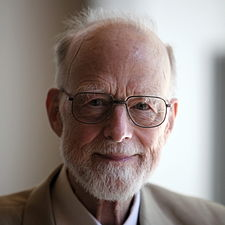
\includegraphics[scale=0.5]{img/TonyHoare.jpg}
\end{center}
\end{frame}

\subsection{Quicksort for C++ implementation}

\begin{frame}[containsverbatim]
\frametitle{}
Here's a typical C++ implementation:
\begin{example}
	\inputminted[linenos=true]{c++}{src/quicksort.cpp}
\end{example}
\end{frame}

\begin{frame}[containsverbatim]
\frametitle{}
Let's summarize
\begin{block}<+->{Disclaimer \#1}
	\vspace{.1cm}
	\large
	The total number of lines is 14
\end{block}
\end{frame}


\begin{frame}[containsverbatim]
\frametitle{}
Here's appropriate Haskell implementation
\begin{example}
	\inputminted[linenos=true]{haskell}{src/quicksort_filter.hs}
\end{example}
Or (the same thing) using list comprehensions
\begin{example}
	\inputminted[linenos=true]{haskell}{src/quicksort_lh.hs}
\end{example}
\end{frame}

\subsection{Comparison of C++ and Haskell}

\begin{frame}[containsverbatim]
\frametitle{}
Let's summarize
\begin{block}<+->{Disclaimer \#2}
	\large
	The total number of lines is 5\\
	The difference between C++ and Haskell version is 14 - 5 = 9 lines !!!
\end{block}
\end{frame}

\subsection{Used Haskell stuff guide 1}

\begin{frame}[containsverbatim]
\frametitle{}
Now let's describe the Haskell implementation of quicksort.\\
But first let's see the result of using quicksort at some sample input data.
\begin{example}
	\inputminted{console}{src/qsort_sample.session}
\end{example}
The numbers in square brackets [] is a regular haskell list (of numbers).\\
But we can sort list of Char-s, Float-s and other types also.\\
\end{frame}


\begin{frame}[containsverbatim]
\frametitle{}
But what is a List from Haskell point of view?
\begin{definition}
	\inputminted{haskell}{src/list_def.hs}
\end{definition}
This is an example of recursively-defined data structure (has no analogs in C++).\\
Here we define a base case - [] for an empty list and a recursive one - item (:) list.
\vspace{.1cm}
And here's some examples with syntactic sugar:
\begin{example}
	\vspace{.1cm}
	\mint{haskell}|[1..3] == [1,2,3] == 1:[2,3] == 1:2:3:[]|
\end{example}
But the Haskell itself always treats is like a degenerated tree
\mint{haskell}|(1:(2:(3:[])))|
\end{frame}


\begin{frame}[containsverbatim]
\frametitle{}
Now it's time to look at the first line of our quicksort:
\begin{definition}
	\mint{haskell}|qsort        :: Ord a => [a] -> [a]|
\end{definition}
This is just a type declaration of qsort function.\\
\begin{itemize}
  \item \mint{haskell}|a| is a type variable (can be Integer, Float, Char, ...).
  \item \mint{haskell}|Ord a =>| is a constraint for the type a (it shold support total ordering).
  \item \mint{haskell}|[a] -> [a]| means that qsort takes a list of some time and return the [sorted] list of the same type.
\end{itemize}
\end{frame}


\begin{frame}[containsverbatim]
\frametitle{}
It worth to be mentioned:
\begin{alertblock}{FYI}
	\begin{itemize}
		\item It's not needed to put type declaration for all the functions.\\
		\item In most cases it will be automatically deduced.\\
		\item According to the Hindley-Milner type inference algorithm.
	\end{itemize}
\end{alertblock}
\end{frame}


\begin{frame}[containsverbatim]
\frametitle{}
Let's look at the Ord type class (corresponds to something like interface in Java/C/C++):
\begin{definition}
	\small
	\inputminted{haskell}{src/ord1.hs}
\end{definition}
\end{frame}


\begin{frame}[containsverbatim]
\frametitle{}
Let's continue:
\begin{definition}
	\small
	\inputminted{haskell}{src/ord2.hs}
\end{definition}
\end{frame}


\begin{frame}[containsverbatim]
\frametitle{}
Before moving to the second line of our quicksort we need to tell about recursive functions definition.
In mathematics we define recursive functions in the following way:
%displaymath
\[
f(n) =
\begin{cases}
1,        & n = 1,\\
n*f(n-1), & n \ge 1
\end{cases}
\]
In Haskell we define it by:
\begin{definition}
\begin{minted}{haskell}
factorial 1 = 1
factorial n = n*factorial(n - 1)
\end{minted}
\end{definition}
Or, using syntax sugar:
\begin{definition}
\begin{minted}{haskell}
factorial n = |n == 1     = 1
              |otherwise  = n*factorial(n - 1)
\end{minted}
\end{definition}
\end{frame}


\begin{frame}[containsverbatim]
\frametitle{}
Now it's time to look at the second line of our quicksort:
\begin{definition}
	\mint{haskell}|qsort []     = []|
\end{definition}
This is just a base-case of a recursively-defined function.\\
If we have an empty list - we don't need to sort it - so let's just return it as a result.\\
\vspace{.1cm}
The third line of our quicksort is:
\begin{definition}
	\mint{haskell}|qsort (x:xs) = (qsort lth) ++ [x] ++ (qsort gth) where|
\end{definition}
This is a recursive case. (x:xs) is a pattern matching of the input list.
Remember the second case of list definition (... a:[a]).
It makes possible to do such pattern-matching around a colon (:) operator.
This is a common trick in FP - split the list to it's head (element) and tail (a smaller list).
\end{frame}


\begin{frame}[containsverbatim]
\frametitle{}
Let's continue with the third line of our quicksort:
\begin{definition}
	\mint{haskell}|qsort (x:xs) = (qsort lth) ++ [x] ++ (qsort gth) where|
\end{definition}
Here [x] is a list of one element - x (for example - [3] or [71]).\\
++ - is a list concatenation operator (sometimes denoted in a literature as \lplus).
\begin{example}
	\inputminted{console}{src/list_concat_sample.session}
\end{example}
(qsort lth) and (qsort gth) is a recursive call with a lists of smaller length.
\end{frame}


\begin{frame}[containsverbatim]
\frametitle{}
Let's continue with the fourth line of our quicksort:
\begin{definition}
	\mint{haskell}|         lth = filter (<  x) xs|
\end{definition}
Here filter is one of the standard Haskell well-known higher-order functions (HOF).\\
In other words - this is a function that takes another functions as it's [first] argument.
\begin{example}
	\inputminted{console}{src/filter_sample.session}
\end{example}
\end{frame}


\begin{frame}[containsverbatim]
\frametitle{}
($<$  x) is a section - partially applied (curried) function for the appropriate operator (x - is the bounded (fixed) second argument).\\
Let's remember Ord type class:
\begin{definition}
	\mint{haskell}|    (<), (<=), (>), (>=) :: a -> a -> Bool|
\end{definition}
All the mentioned functions (operators) takes 2 arguments.\\
But if we fix (partially apply) one of the argument - the remaining function will be of one argument which returns Bool (True $\vert$ False).
\begin{example}
	\inputminted{console}{src/section_sample.session}
\end{example}
\end{frame}


\begin{frame}[containsverbatim]
\frametitle{}
Here's a definition of standard (Prelude) version of filter higer-order (HOF) function:
\begin{definition}
	\inputminted{haskell}{src/filter_hof.hs}
\end{definition}
\end{frame}


\begin{frame}[containsverbatim]
\frametitle{}
The type declaration of filter tells us that it's a HOF by the bracket around the first argument:\\
\mint{haskell}|filter :: (a -> Bool) -> ...|
The second argument is a list of type \textbf{a} ([a])\\
The result is also the list of typa \textbf{a} which contains the same or fewer elements than the second argument.
The next line of filter definition:
\mint{haskell}|filter _pred []    = []|
Is a partial definition for the case then the second argument is an empty list.\\
The first argument (predicate \textbf{\_pred}) does not matter in this case.
It is usual to user the underscore symbol - \_ for such cases.
\end{frame}


\begin{frame}[containsverbatim]
\frametitle{}
The other lines of filter definition is a recursive case:
\begin{minted}{haskell}
filter pred  (x:xs)
  | pred x         = x : filter pred xs
  | otherwise      = filter pred xs
\end{minted}
It consists of two parts.\\
The first one is for the case if predicate \textbf{pred} is \textbf{True} for the element \textbf{x}.
In this case we keep the element \textbf{x}.\\
\mint{haskell}|x : filter pred xs|
The second one (\textbf{otherwise}) is for for the opposite case (\textbf{False}).
In this case we skeep(omit) \textbf{x}.
\mint{haskell}|filter pred xs|
And process a list of the smaller size (\textbf{xs}) recursively.
\end{frame}


\section{Other Famous Higher-Order Functions}

\subsection{Map-Reduce(Fold)}


\begin{frame}[containsverbatim]
\frametitle{}
We've just finished with one of the most famous HOF: filter. But there are also other two ones,
\textbf{greately} used in functional programming.\\
But first let's not break a tradition and start from example.\\
Let's summarize the squares of all the natural numbers starting from one up to \textbf{n}.
\[1^2 + 2^2 + ... n^2\]
For the C++ this would be:
\begin{example}
	\inputminted[linenos=true]{c++}{src/sumnats.cpp}
\end{example}
\end{frame}


\begin{frame}[containsverbatim]
\frametitle{}
For the Haskell this function will be much simpler (\textbf{AGAIN!}):
\begin{example}
	\inputminted[linenos=true]{haskell}{src/sumnats.hs}
\end{example}
The comparison is:
\begin{block}<+->{Disclaimer \#2}
	\large
	The total number of lines for the C++ case is 5\\
	The total number of lines for the Haskell case is 2\\
	The difference between C++ and Haskell version is 7 - 2 = 5 lines !!!
\end{block}
\end{frame}


\begin{frame}[containsverbatim]
\frametitle{}
The list comprenehsion [1..n] is just a syntax sugar for the list of successive numbers from 1 to n. \\
Consider the case n = 5:
\begin{example}
	\inputminted{console}{src/simple_list_comprehension_1_5.session}
\end{example}
Now let's describe the following sub-expression:
\mint{haskell}|map (\x -> x^2) [1..n]|
The map HOF - is for applying it's first argument (function) to the list.
\begin{example}
	\inputminted{console}{src/map_square_1_5.session}
\end{example}
\end{frame}


\begin{frame}[containsverbatim]
\frametitle{}
Here's a more general description of map:
\begin{definition}
\begin{minted}{haskell}
map f [x1, x2, ..., xn] == [f x1, f x2, ..., f xn]
map f [x1, x2, ...] == [f x1, f x2, ...]
\end{minted}
\end{definition}
And this is the formal (source code) definition of map:
\begin{definition}
	\inputminted{haskell}{src/map_hof.hs}
\end{definition}
We pattern-match on a list constructor (:), convert matching element using f-function
and process the rest of the list (xs) recursively.
\end{frame}


\begin{frame}[containsverbatim]
\frametitle{}
The foldr (as well as foldl) is the most famous HOF - for traversing elements of the list from right (to left)
starting from a specified element (0 in our case):
\begin{example}
	\inputminted{console}{src/foldr_square_1_5.session}
\end{example}
Here's a more general description of foldr:
\begin{definition}
\begin{minted}{haskell}
foldr (op) x0 [x1, x2, ..., xn] ==
  (x1 'op' (x2 'op' ... 'op' (xn 'op' x0)))
-- or, in case of associative operation 'op':
foldr (op) x0 [x1, x2, ..., xn] ==
  x1 'op' x2 'op' ... 'op' xn 'op' x0
\end{minted}
\end{definition}
\end{frame}


\begin{frame}[containsverbatim]
\frametitle{}
In graphical form, foldr and foldl can be represented as:
\begin{tabular}{p{0.5\textwidth} p{0.5\textwidth}}
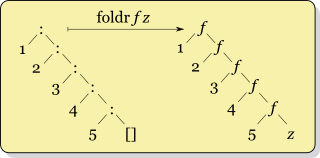
\includegraphics[scale=0.5]{img/Right-fold-transformation.png} &
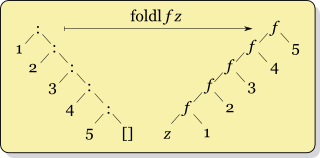
\includegraphics[scale=0.5]{img/Left-fold-transformation.png} \\
\end{tabular}
In other words - we replace the empty list ([]) by start element and list constructor (:)
by our operation.\\
And this is the formal (source code) definition of foldr:
\begin{definition}
	\inputminted{haskell}{src/foldr_hof.hs}
\end{definition}
\end{frame}


\begin{frame}[containsverbatim]
\frametitle{}
Another sample - let's calculate a maximum of list elements.\\
Traditional (C++) approach is:
\begin{example}
	\inputminted[linenos=true]{c++}{src/max_for_list.cpp}
\end{example}
The haskell version is:
\begin{example}
	\inputminted[linenos=true]{haskell}{src/max_for_list.hs}
\end{example}
\end{frame}


\begin{frame}[containsverbatim]
\frametitle{}
Here foldr1 is a standard Haskell derivation of foldr (using last element of a list as a start one):
\begin{definition}
	\inputminted[linenos=true]{haskell}{src/foldr1_hof.hs}
\end{definition}
\end{frame}


\begin{frame}[containsverbatim]
\frametitle{Fold Universality}
Fold is a very universal. Map can be expressed through it:
\mint{haskell}|map' f xs = foldr ((:) . f) []) xs|
Haskell allows to omit all the dupclicated arguments if they appear at the both (left and right) side of definition:
\mint{haskell}|map' f = foldr ((:) . f) [])|
This is called point-free style.\\
((:) . f) is a composition of list constructor (:) and argument-function f. Function composition (.) is defined as:
\begin{minted}{haskell}
(.) :: (b -> c) -> (a -> b) -> (a -> c)
(.) f g = \x -> f (g x)
\end{minted}
The last line can be also written as:
\mint{haskell}|f . g = \x -> f (g x)|
\end{frame}


\begin{frame}[containsverbatim]
\frametitle{}
Filter can be represented as:
\begin{minted}{haskell}
filter' :: (a -> Bool) -> [a] -> [a]
filter' p = foldr (\x acc -> if p x then x : acc else acc) []
\end{minted}
Note: If always have the else-clause in haskell since it's pure functional language (without side-effects).
\end{frame}


\begin{frame}[containsverbatim]
\frametitle{}
Many list functions can be specified by a single foldr:
\begin{example}
\[
%\begin{aligned}
\begin{array}{lll}
sum     &=& foldr \medspace (+)                          \medspace 0         \\
product &=& foldr \medspace (*)                          \medspace 1         \\
and     &=& foldr \medspace (\land)                      \medspace True      \\
or      &=& foldr \medspace (\lor)                       \medspace False     \\
maximum &=& foldr \medspace max                          \medspace (-\infty) \\
minimum &=& foldr \medspace min                          \medspace \infty    \\
length  &=& foldr \medspace (\lambda \_ n \mapsto 1 + n) \medspace 0         \\
concat  &=& foldr \medspace (\lplus)                     \medspace []        \\
\end{array}
\]
\end{example}
\end{frame}


\begin{frame}[containsverbatim]
\frametitle{}
The Bird-Meertens Formalism, devised by Richard Bird and Lambert Meertens:
\begin{itemize}
	\item The BMF (also called Squiggol) is a calculus for deriving programs from specifications (in a functional program setting).
	\item Proposes algebra of List-based data structures with map/fold/filter HOFs, composition and primitive operations.
	\item A big class of regular loop/for calculations in imperative languges can be easily described by BMF.
	\item List-functions, calculated this way (homomorphisms), can be easily parallelized (Map/Reduce).
\end{itemize}
The great introduction to Lists, Monoids, Homomorphisms (and it's 3 theorems) is given in russian at 
{\color{Blue} \href{http://habrahabr.ru/blogs/programming/126275}{Folds in Intel Click Plus} } article.
\end{frame}


\begin{frame}[containsverbatim]
\frametitle{Selected Publications}
\begin{table}[t]
	\begin{tabular}{ccc}
		Richard Bird & Lambert Meertens & Jeremy Gibbons\\
		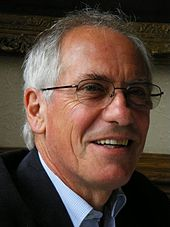
\includegraphics[width=1.5cm]{img/RichardSBird.jpg} &
		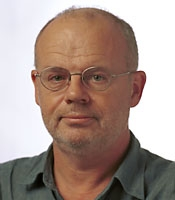
\includegraphics[width=1.5cm]{img/LambertMeertens.jpg} &
		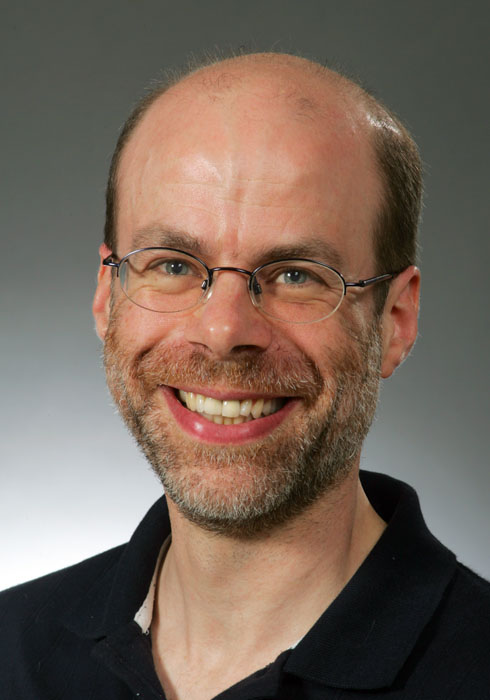
\includegraphics[width=1.5cm]{img/JeremyGibbons.jpg} \\
	\end{tabular}
\end{table}

\begin{itemize}
	\item {\color{Blue} \href{http://www.cs.ox.ac.uk/files/3378/PRG56.pdf}{R.S. Bird, An Introduction to the theory of lists} }
	\item {\color{Blue} \href{http://www.kestrel.edu/home/people/meertens/publications/papers/Algorithmics.pdf}{Lambert Meertens. Algorithmics � Towards programming as a mathematical activity} }
	\item {\color{Blue} \href{http://web.comlab.ox.ac.uk/people/Jeremy.Gibbons/publications/thirdht.ps.gz}{Jeremy Gibbons. The Third Homomorphism Theorem} }
\end{itemize}
\end{frame}


\section{Safety}


\begin{frame}[containsverbatim]
\frametitle{Safety}
Consider the case - we need to describe a flock of sheep. Every sheep has a mother and father.
In C++ we usually write this:
\begin{minted}{c++}
class Sheep {
public:
  std::string m_Name;
  Sheep      *m_pFather;
  Sheep      *m_pMother;

  Sheep(const std::string &name)
  : m_Name(name), m_pFather(NULL), m_pMother(NULL)
  {}
}
\end{minted}
And if we need to get a name of the fater we write:
\mint{c++}|std::string fater_name = aSheep.pFater->name|
And this is sometimes {\color{Red} JUST CRASH with ACCESS VIOLATION} since aSheep can be
a "Dolly-clone" without mother and/or father.
\end{frame}


\begin{frame}[containsverbatim]
\frametitle{Safety}
"Null References" are also invented by C.A.R. Hoare.\\
\begin{block}{Citation}
\footnotesize
I call it my billion-dollar mistake. It was the invention of the null reference in 1965.
At that time, I was designing the first comprehensive type system for references in an
object oriented language (ALGOL W).\\
My goal was to ensure that all use of references should be absolutely safe, with checking
performed automatically by the compiler. But I couldn't resist the temptation to put in a
null reference, simply because it was so easy to implement.\\
This has led to innumerable errors, vulnerabilities, and system crashes, which have probably
caused a billion dollars of pain and damage in the last forty years.\\
In recent years, a number of program analysers like PREfix and PREfast in Microsoft have been used
to check references, and give warnings if there is a risk they may be non-null.
More recent programming languages like Spec\# have introduced declarations for non-null references.\\
This is the solution, which I rejected in 1965. 
\end{block}
\end{frame}


\begin{frame}[containsverbatim]
\frametitle{Nulls at Haskell}
In haskell there is no such notion as null. It uses Maybe algebraic data type (ADT) in order to represent
calculation which may provide no any result:
\begin{example}
	\inputminted{haskell}{src/maybe_adt.hs}
\end{example}
Here "Maybe" is a type-constructor function (it gives a type "a" as an input and returns a new type
"Maybe a").\\
"Nothing" and "Just a" are value constructors.
\end{frame}


\begin{frame}[containsverbatim]
\frametitle{Nulls at Haskell}
Datatype for our sheep is:
\begin{example}
	\inputminted{haskell}{src/sheep.hs}
\end{example}
\end{frame}

\begin{frame}[containsverbatim]
\frametitle{Nulls at Haskell}
The following function will find mothernal grandfather:
\begin{example}
	\inputminted{haskell}{src/sheep_grands.hs}
\end{example}
Let's try to forget about "Nothing" case:
\begin{example}
	\inputminted{haskell}{src/sheep_grands-nothing-commented.hs}
\end{example}
\end{frame}


\begin{frame}[containsverbatim]
\frametitle{Nulls at Haskell}
Let's compile the mentioned version:
\begin{example}
	\inputminted{console}{src/pattern_match_warning.session}
\end{example}
We can see that the compiler warns us about incomplete case alternatives.\\
Note: this works only if we are interesting in warning (-Wall option).
\end{frame}


\section{Monads}
\subsection{Problematic case}


\begin{frame}[containsverbatim]
\frametitle{Nulls at Haskell}
But what if we need to know a more distant ancestor?
The typical solution is to use a nested case operators (or if-then-else):
\begin{example}
	\inputminted{haskell}{src/sheep_grands_grands.hs}
\end{example}
How does Haskell deal with this issue?\\
The answer is - MONADS !!!
\end{frame}


\subsection{Glue function togeather}


\begin{frame}[containsverbatim]
\frametitle{Do you see similarity?}
Let's look on the following very similar functions:\\
\begin{example}
	\inputminted{haskell}{src/sheep_samples.hs}
\end{example}
\end{frame}


\begin{frame}[containsverbatim]
\frametitle{Unusual functional composition}
They all are ALMOST the same except having \textit{\textbf{mother}} and \textit{\textbf{father}} at distinct places.\\
This means that we can ABSTRACT from the function specific (\textit{\textbf{mother}} or \textit{\textbf{father}}
which are of the same type) and think about function composition in an UNUSUAL way.
\begin{example}[unusual functional composition]
	\inputminted{haskell}{src/sheep_compose_1.hs}
\end{example}
\end{frame}


\begin{frame}[containsverbatim]
\frametitle{Great simplification}
Using our unusual composition \textit{\textbf{s\_comp}} we can GREATLY simplify our functios:
\begin{example}[great simplification]
	\inputminted{haskell}{src/sheep_compose_2.hs}
\end{example}
\end{frame}


\begin{frame}[containsverbatim]
\frametitle{Why is this unusual?}
Why is this kind of composition is UNUSUAL?\\
Let's remember the usual function composition:
\begin{example}[usual functional composition]
\begin{minted}{haskell}
(.) :: (b -> c) -> (a -> b) -> (a -> c)
(.) f g = \x -> f (g x)
\end{minted}
\end{example}
In a usual way (using point in Haskell) we can combine two functions such that the input argument type (\textbf{domain})
of the first is equal to the output (\textbf{domain}) of the other (type-variable "b" at the example).\\
Returning to our SHEEPs, we need to compose functions, domen of the first one (Sheep) is NOT-EQUAL
to the codomain of the second (Maybe Sheep).\\
That's why our sheep-function-composition is UNUSUAL.
\end{frame}


\subsection{Monadic functions}


\begin{frame}[containsverbatim]
\frametitle{Monadic functions}
So, our sheep-functions (of type "Sheep $->$ Maybe Sheep") are called \textbf{monadic-functions}.\\
For 's\_comp' Haskel uses special fish-operator ($>=>$).
\begin{alertblock}{Haskell syntax}
\small
In Haskell operator is a function named by spec-symbols only.\\
Regular function names are made of of alpha-numeric symbols only (first is alpha).
Mixing spec-symbols and alpha-numberic symbols is prohibited.\\
Operators are used in infix form by default, but can be written in prefix form togeather with parenthesis:
\begin{minted}{haskell}
plus x y = x + y
minus x y = (-) x y
\end{minted}
Regular functions are in prefix form by default, but can be written in infix form togeather with quotes:
\begin{minted}{haskell}
mean x y = (plus x y) / 2
mean x y = (x 'plus' y) / 2
\end{minted}
\end{alertblock}
\end{frame}


\subsection{Monadic fish operator}


\begin{frame}[containsverbatim]
\frametitle{Monadic fish-operator}
Abstracting from "Maybe" (replacing it by "m") we can write the type of our fish operator (for our simple case) as:
\mint{haskell}|(>=>) :: Monad m => (a -> m a) -> (a -> m a) -> (a -> m a)|
Remember, that in our case "a" stands for "Sheep", and "m" stands for "Maybe".\\
So, it gives two monadic functions, glues them togeather and returns a new monadic function (all are of the same type).\\
In Haskell in order to be a (\textbf{Monad}), fish-operator MUST be associative (for Maybe case):
\mint{haskell}|(f >=> g) >=> h  ==  f >=> (g >=> h)|
Please, try to prove (or find in google) that fish is really associative for the case of "Maybe".
\end{frame}


\begin{frame}[containsverbatim]
\frametitle{Monadic fish-operator}
\begin{block}{Proof hints}
Glueing maybe--monadic-functions we always propagate "Nothing" case (no matter at what position).\\
If all the values are in a "Just x" form - we get a regular function composition, which is known to be associative.
\end{block}
Taking associativeness in account we are free to omit parenthesis:
\begin{example}
\mint{haskell}|motPatGrand = mother >=> father >=> father|
\end{example}
So, monadic fish-operator (as a first approximation) forms a semigroup at the set of monadic functions.
\begin{alertblock}{Algebra goes into play}
From this moment we can use ALGEGRAIC methods while operating with monads.
\end{alertblock}
\end{frame}


\subsection{Monadic return operator}


\begin{frame}[containsverbatim]
\frametitle{Combining monadic with non-monadic function}
But how can we combine a regular and monadic function ?\\
Suppose we have the following function for making a brother of the Sheep:
\begin{example}
\begin{minted}{haskell}
brother :: Sheep -> Sheep
brother s = Sheep(
  name(s) ++ "_brother"
  mother(s)
  father(s)
)
\end{minted}
\end{example}
It returns a plain \textbf{Sheep} (not a \textbf{Maybe Sheep}).\\
So, we need a kind of CONNECTOR function (to convert from plain \textbf{Sheep} to a \textbf{Maybe Sheep}).
\end{frame}


\begin{frame}[containsverbatim]
\frametitle{Monadic return function}
In Haskell a function named \textbf{return} is used for such convertion.\\
\begin{example}
\begin{minted}{haskell}
return :: Sheep -> Maybe Sheep
return s = Just s
\end{minted}
\end{example}
It gives a Sheep s and return a Just value-constructor for it.\\
Now we can combine our \textbf{brother} function with just defined \textbf{return} in order to get
a monadic function:
\begin{example}
\begin{minted}{haskell}
monadic_brother :: Sheep -> Maybe Sheep
monadic_brother = return . brother
\end{minted}
\end{example}
We just used a regular composition (.) and Haskell point-free style here.
\end{frame}


\begin{frame}[containsverbatim]
\frametitle{Monoid}
Since return does nothing with its argument except placing it into Maybe monad, we can easily
check the following statements:
\begin{example}
\begin{minted}{haskell}
fun >=> return  ==  fun
return >=> fun  ==  fun
\end{minted}
\end{example}
In other words, return - is the identity element for monadic fish-composition at the set of \textit{simple}
monadic functions.\\
So, our \(>=>\) and return form a Monoid (semigroup with identity element OR group without inversibility).
\begin{alertblock}{Algebra goes into play}
We continue using ALGEGRAIC methods while operating with monads.
\end{alertblock}
\end{frame}


\subsection{Types correction}


\begin{frame}[containsverbatim]
\frametitle{Correcting monadic composition}
Let's remind our regular function composition:
\begin{example}[usual functional composition]
\begin{minted}{haskell}
(.) :: (b -> c) -> (a -> b) -> (a -> c)
(.) f g = \x -> f (g x)
\end{minted}
\end{example}
Our simplistic-version of monadic composition was:
\mint{haskell}|(>=>) :: Monad m => (a -> m a) -> (a -> m a) -> (a -> m a)|
Actually in Haskell, fish has more sophisticated type:
\mint{haskell}|(>=>) :: Monad m => (a -> m b) -> (b -> m c) -> (a -> m c)|
There is also a flipped-version of fish-operator (similar to regular composition):
\mint{haskell}|(<=<) :: Monad m => (b -> m c) -> (a -> m b) -> (a -> m c)|
\end{frame}


\begin{frame}[containsverbatim]
\frametitle{Correcting monadic composition}
So, what is a regular function composition?\\
Let's call \(F_1\) a set of all the one-argument functions:
\[F_1 = \{ f : A \mapsto B \}\]
Then, composition can be treated as a partial function from cartesian product of \(F_1\) with itself to \(F_1\).
\[\circ : (F_1 \times F_1) \pfun F_1\]
In the same way, monadic fish composition operator is also a partial function (not all the monadic functions
can be combined with it, but only those that match type constraints).
\end{frame}


\subsection{Monads in Haskell}


\begin{frame}[containsverbatim]
\frametitle{Monad type class}
Taking all the above into account, the question is - "What is a monad in Haskell"?
Let's look at the source code:
\begin{example}
	\small
	\inputminted{haskell}{src/monad_typeclass.hs}
\end{example}
\end{frame}


\begin{frame}[containsverbatim]
\frametitle{Fish and Bind operators}
Let's compare the monadic bind-operator and a fish-one:
\begin{example}
	\small
	\inputminted{haskell}{src/fish_hof.hs}
\end{example}
So, fish-operator is a polymorphic higher-order function, defined for ALL the monads through the
appropriate SPECIFIC bind operator.
\end{frame}


\subsection{Maybe-monad}


\begin{frame}[containsverbatim]
\frametitle{Fish and Bind for Maybe}
The Maybe monad in Haskell is defined as:
\begin{example}
	\small
	\inputminted{haskell}{src/maybe_monad.hs}
\end{example}
\end{frame}


\subsection{Monad-laws}


\begin{frame}[containsverbatim]
\frametitle{Monad laws - nice version}
As we told above, in order to be a monad, a programmer (not a compiler) MUST enforce the followin LAWS for specific monad.\\
The nice version of monad laws uses fish-operator:
\begin{example}
	\small
	\inputminted{haskell}{src/monad_laws_nice.hs}
\end{example}
Compare with the composition LAWS:
\begin{example}
	\small
	\inputminted{haskell}{src/composition_laws.hs}
\end{example}
What is the difference ???
\end{frame}


\begin{frame}[containsverbatim]
\frametitle{Monad laws - ugly version}
The UGLY version of the same laws is using monadic bind operator:
\begin{example}
	\small
	\inputminted{haskell}{src/monad_laws_ugly.hs}
\end{example}
Ensuring the correctness of monad laws for standard/custom monads is CRITICAL for the correctness since Haskell
compiler is free to evaluate fish/bind operators in ANY ORDER!!!
\end{frame}


\subsection{Monad-folding}


\begin{frame}[containsverbatim]
\frametitle{Monad folding}
What if we need to compose a dynamic list of monadic functions?
\begin{example}
	\small
	\mint{haskell}|h = mf1 >=> mf2 >=> ... >=> mfN|
\end{example}
In this case we need to use a folding function (foldr or foldl):
\begin{example}
	\small
	\mint{haskell}|h = foldr (>=>) return [mf1, mf2, ..., mfN]|
\end{example}
Remember that:
\begin{itemize} %\mathbf \boldsymbol \pmb, package{bm} -> \bm
  \item \textbf{return} is an identity element of our monoid
  \item fish-operator (\boldmath$>=>$) - operation of monoid (semigroup)
  \item monadic functions (\textbf{mf1, mf2, ... mfN}) - elements of monoid
\end{itemize}
\begin{block}{S.McLane}
Monad is the Monoid at the category of endofunctors.
\end{block}
\end{frame}


\subsection{List comprehensions}


\begin{frame}[containsverbatim]
\frametitle{List comprehensions - Intro}
It's time to remember our first example - quicksort function.
\begin{example}
	\small
	\inputminted{haskell}{src/quicksort_lh.hs}
\end{example}
The expression in square brackets is a Haskell \textbf{list comprehension}.\\
\end{frame}


\begin{frame}[containsverbatim]
\frametitle{Pythagorean triples}
Let's find all the positive triples such that \(x^2 + y^2 = z^2\).\\
C++0x version (n is the limit) is:
\begin{example}
	\small
	\inputminted{c++}{src/pyth_triple.cpp}
\end{example}
\end{frame}


\begin{frame}[containsverbatim]
\frametitle{Pythagorean triples in Haskell}
Haskell version with list comprehensions is:\\
\begin{example}
	\small
	\inputminted{haskell}{src/pyth_triple_lc.hs}
\end{example}
Sample session (for n = 20):
\begin{example}
	\small
	\inputminted{console}{src/pyth_20.session}
\end{example}
List comprehensions actually is a very conveniet syntax sugar over \textbf{List Monad}.
\end{frame}


\begin{frame}[containsverbatim]
\frametitle{Pythagorean triples desugared}
So, desugared version of pythagorean triples uses list monad:
\begin{example}
	\small
	\inputminted{haskell}{src/pyth_triple_list_monad.hs}
\end{example}
Do-notation is also just a syntactic sugar with the following rules
\begin{definition}
	\small
	\inputminted{haskell}{src/do_notation_rules.hs}
\end{definition}
\end{frame}


\begin{frame}[containsverbatim]
\frametitle{Desugared List monad}
Desugared version using monadic bind operator is:
\begin{example}
	\scriptsize %\tiny \footnotesize
	\inputminted{haskell}{src/pyth_triple_desugared.hs}
\end{example}
Here guard - is a monadic higher-order function:
\begin{example}
	\small
	\inputminted{haskell}{src/guard_hof.hs}
\end{example}
\end{frame}


\subsection{Monad Plus}


\begin{frame}[containsverbatim]
\frametitle{MonadPlus}
MonadPlus class extends Monad in order to support choice and failure:
\begin{example}
	\scriptsize %\tiny \footnotesize
	\inputminted{haskell}{src/monadplus_class.hs}
\end{example}
\end{frame}


\subsection{List Monad}


\begin{frame}[containsverbatim]
\frametitle{List Monad}
And, finally, list monad is defined as:
\begin{example}
	\small %\tiny \footnotesize
	\inputminted{haskell}{src/list_monad.hs}
\end{example}
Here return is an identity monadic function (of type a $\mapsto$ [a]).\\
It just puts an argument to the list (returns a one-elemen-list).
\smallskip \par %\smallskip \medskip \bigskip
Function f (also of a type a $\mapsto$ [b]) is any monadic function.\\
It converts an argument to the list of some type (equal or not to the type of argument).
\smallskip \par
Bind maps \textbf{f} over monadic value (xs list) which leads to the list of lists, 
then - makes a plain version via concat function.
\end{frame}


\begin{frame}[containsverbatim]
\frametitle{List Monad Bind example}
In order to be more clear, consider example:
\begin{example}
	\small
	\inputminted{console}{src/list_bind.session}
\end{example}
Concat is defined as:
\begin{example}
	\small
	\inputminted{haskell}{src/concat_hof.hs}
\end{example}
\end{frame}


\subsection{Powerset example}


\begin{frame}[containsverbatim]
\frametitle{Powerset definition}
Consider the powerset - set of all subsets of the given set.\\
For simplicity let original set be all numbers from 0 to N-1.\\
For N = 4 the set will be {0,1,2,3} and its powerset:
\begin{example}
	\tiny
	\inputminted{console}{src/powerset_4.session}
\end{example}
\end{frame}


\begin{frame}[containsverbatim]
\frametitle{Powerset in c++ - part 1}
Another example - all subsets of the given set (powerset):
\begin{example}
	\small
	\inputminted{c++}{src/powerset1.cpp}
\end{example}
\end{frame}


\begin{frame}[containsverbatim]
\frametitle{Powerset in c++ - part 2}
Calling the powerset (in CPS style using C++0x lambdas):
\begin{example}
	\small
	\inputminted{c++}{src/powerset2.cpp}
\end{example}
\end{frame}


\begin{frame}[containsverbatim]
\frametitle{Powerset in Haskell}
In Haskell the powerset is:
\begin{example}
	\small
	\inputminted{haskell}{src/powerset.hs}
\end{example}
Here's a standard polymorphic monadic HOF filterM:
\begin{example}
	\small
	\inputminted{haskell}{src/filterM_hof.hs}
\end{example}
\end{frame}


\begin{frame}[containsverbatim]
\frametitle{Questions}
Additional stuff:
\begin{itemize}
	\item {\color{Blue} \href{https://github.com/iharh/fp-by-example}{TeX sources at github} }
\end{itemize}
\end{frame}

\end{document}
